\documentclass[tikz,border=2pt]{standalone}
\usetikzlibrary{calc}
\usetikzlibrary{intersections}
\usetikzlibrary{patterns}
\usepackage{bm}
\usetikzlibrary{positioning}
\usetikzlibrary{shapes}

\begin{document}

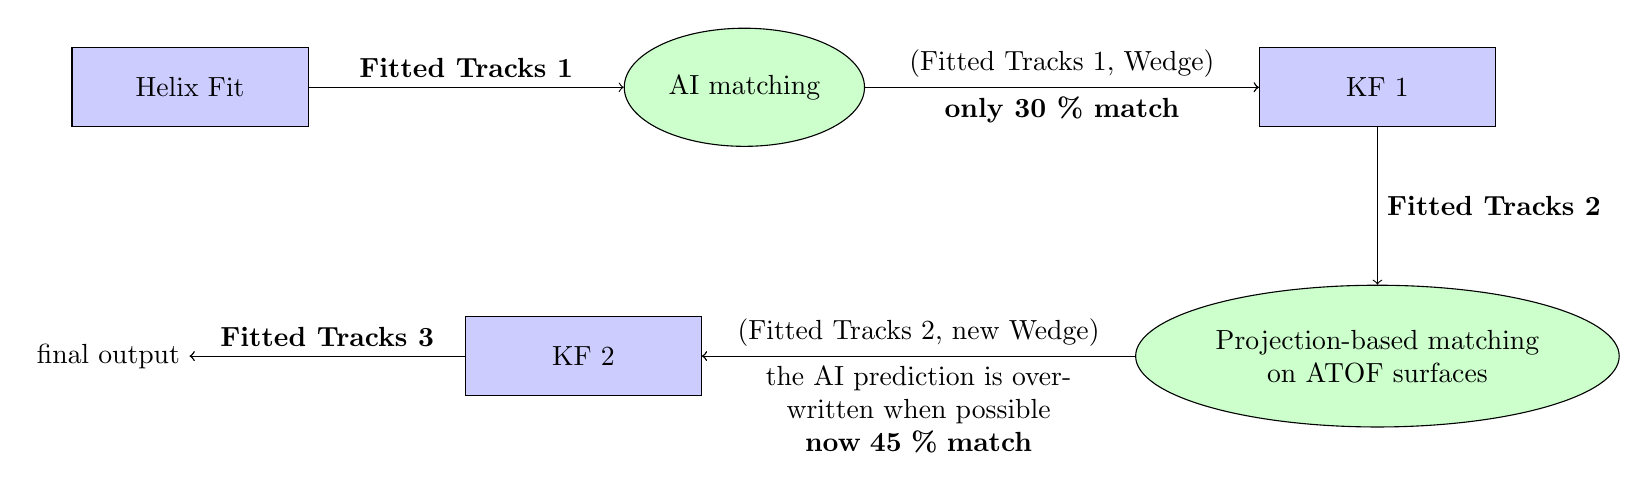
\begin{tikzpicture}
    
    % Helix Fit
    \node[draw, rectangle, fill=blue!20, minimum width=3cm, minimum height=1cm] (A) {Helix Fit};
    % AI matching
    \node[draw, shape=ellipse,minimum height=1.5cm, fill=green!20, right=4cm of A] (B) {AI matching};
    \draw[->] (A) -- node[midway, above]{\bf Fitted Tracks 1} (B);
    % KF1
    \node[draw, rectangle, fill=blue!20, minimum width=3cm, minimum height=1cm, right=5cm of B] (C) {KF 1};
    \draw[->] (B) -- node[midway, above]{(Fitted Tracks 1, Wedge)} (C);
    \draw[->] (B) -- node[midway, below]{\bf only 30 \% match} (C);
    % Projection
    \node[draw, shape=ellipse,minimum height=1.8cm, below=2cm of C, align=center, fill=green!20] (D) {Projection-based matching\\ on ATOF surfaces};
    \draw[->] (C) -- node[midway, right]{\bf Fitted Tracks 2} (D);
    % KF1
    \node[draw, rectangle, fill=blue!20, minimum width=3cm, minimum height=1cm, left=5.5cm of D] (E) {KF 2};
    \draw[->] (D) -- node[midway, above]{(Fitted Tracks 2, new Wedge)} (E);
    \draw[->] (D) -- node[midway, below, align=center, text width=5cm]{the AI prediction is overwritten when possible\\\bf now 45 \% match} (E);
    % final ouput
    \draw[->] (E) -- node[midway, above]{\bf Fitted Tracks 3} ++(-5cm,0);
    \draw[->] (E) -- ++(-5cm,0) node [left] {final output};
    
    
    

\end{tikzpicture}


\end{document}